In this chapter, the results of several large-scale simulations are presented. 

More specifically, 2D3V PIC simulations of tightly-focused Gaussian laser beams interacting with solid targets have been performed within this work. Simulations have been computed using code EPOCH (see chapter 3). 

\noindent
Zeroth set (4 simulations with const. E = 2.8306e4 J, traget 2 micron, 2000 ppc):
\noindent
Laser:
\begin{itemize}
	\item wavelength: $ \lambda $ = 0.8 $ \mu m $
	\item const. energy: E = 2.8306e4 J (corresponds to I = 1e20 W/cm2 for $ w_0 $ = 1.0 $ \mu m $)
	\item duration: t = 30 fs (in FWHM)
	\item beam waist in focus: $ w_0 $ = 0.5, 1.0, 2.0, 4.0 $ \mu m $
	\item focus distance from boundary: $ x_\mathrm{B} - x_0 $ = 8 $ \mu m $
	\item polarization: P
	\item boundary: left 
\end{itemize}
Domain:
\begin{itemize}
	\item x min: 0 $ \mu m $
	\item x max: 15 $ \mu m $
	\item y min: -20 $ \mu m $
	\item y max: 20 $ \mu m $
	\item $ N_x $: 1875 cells ($ \delta x $ = $ \lambda/100 $ = 8 nm)
	\item $ N_y $: 5000 cells ($ \delta y $ = $ \lambda/100 $ = 8 nm)
	\item time step: $ \delta t $ = $ 1/(\sqrt{2} c) \lambda /100 \approx $ 0.05 fs 
	\item simulation time: $ \tau $ = 200 fs
\end{itemize}
Target:
\begin{itemize}
	\item x min: 8 $ \mu m $
	\item x max: 10 $ \mu m $
	\item y min: -15 $ \mu m $
	\item y max: 15 $ \mu m $
	\item electrons: 2000 ppc
	\item protons: 100 ppc
	\item density: 100 critical
	\item temperature: 100 eV
\end{itemize}

\noindent
First set (4 simulations with const. I = 1e20 W/cm2, traget 2 micron, 2000 ppc):
\noindent
Laser:
\begin{itemize}
	\item wavelength: $ \lambda $ = 0.8 $ \mu m $
	\item const. intensity: I = 1e20 W/cm2
	\item duration: t = 30 fs (in FWHM)
	\item beam waist in focus: $ w_0 $ = 0.5, 1.0, 2.0, 4.0 $ \mu m $
	\item focus distance from boundary: $ x_\mathrm{B} - x_0 $ = 8 $ \mu m $
	\item polarization: P
	\item boundary: left 
\end{itemize}
Domain:
\begin{itemize}
	\item x min: 0 $ \mu m $
	\item x max: 15 $ \mu m $
	\item y min: -20 $ \mu m $
	\item y max: 20 $ \mu m $
	\item $ N_x $: 1875 cells ($ \delta x $ = $ \lambda/100 $ = 8 nm)
	\item $ N_y $: 5000 cells ($ \delta y $ = $ \lambda/100 $ = 8 nm)
	\item time step: $ \delta t $ = $ 1/(\sqrt{2} c) \lambda /100 \approx $ 0.05 fs 
	\item simulation time: $ \tau $ = 200 fs
\end{itemize}
Target:
\begin{itemize}
	\item x min: 8 $ \mu m $
	\item x max: 10 $ \mu m $
	\item y min: -15 $ \mu m $
	\item y max: 15 $ \mu m $
	\item electrons: 2000 ppc
	\item protons: 100 ppc
	\item density: 100 critical
	\item temperature: 100 eV
\end{itemize}

\noindent
Seconds set (4 simulations with const. I = 1e21, 1000 ppc):
\noindent
Laser:
\begin{itemize}
	\item wavelength: $ \lambda $ = 0.8 $ \mu m $
	\item const intensity: I = 1e21 W/cm2
	\item duration: t = 30 fs (in FWHM)
	\item beam waist in focus: $ w_0 $ = 0.5, 1.0, 2.0, 4.0 $ \mu m $
	\item focus distance from boundary: $ x_\mathrm{B} - x_0 $ = 8 $ \mu m $
	\item polarization: P
	\item boundary: left 
\end{itemize}
Domain:
\begin{itemize}
	\item x min: 0 $ \mu m $
	\item x max: 15 $ \mu m $
	\item y min: -20 $ \mu m $
	\item y max: 20 $ \mu m $
	\item $ N_x $: 1875 cells ($ \delta x $ = $ \lambda/100 $ = 8 nm)
	\item $ N_y $: 5000 cells ($ \delta y $ = $ \lambda/100 $ = 8 nm)
	\item time step: $ \delta t $ = $ 1/(\sqrt{2} c) \lambda /100 \approx $ 0.05 fs 
	\item simulation time: $ \tau $ = 200 fs
\end{itemize}
Target:
\begin{itemize}
	\item x min: 8 $ \mu m $
	\item x max: 10 $ \mu m $
	\item y min: -15 $ \mu m $
	\item y max: 15 $ \mu m $
	\item electrons: 1000 ppc
	\item protons: 100 ppc
	\item density: 100 critical
	\item temperature: 100 eV
\end{itemize}

\noindent
Third set (2 simulations with I = 1e21 W/cm2, thiner target (0.25 micron), 2000 ppc):
\noindent
Laser:
\begin{itemize}
	\item wavelength: $ \lambda $ = 0.8 $ \mu m $
	\item const intensity: I = 1e21 W/cm2
	\item duration: t = 30 fs (in FWHM)
	\item beam waist in focus: $ w_0 $ = 0.5, 2.0 $ \mu m $
	\item focus distance from boundary: $ x_\mathrm{B} - x_0 $ = 8 $ \mu m $
	\item polarization: P
	\item boundary: left 
\end{itemize}
Domain:
\begin{itemize}
	\item x min: 0 $ \mu m $
	\item x max: 15 $ \mu m $
	\item y min: -20 $ \mu m $
	\item y max: 20 $ \mu m $
	\item $ N_x $: 1875 cells ($ \delta x $ = $ \lambda/100 $ = 8 nm)
	\item $ N_y $: 5000 cells ($ \delta y $ = $ \lambda/100 $ = 8 nm)
	\item time step: $ \delta t $ = $ 1/(\sqrt{2} c) \lambda /100 \approx $ 0.05 fs 
	\item simulation time: $ \tau $ = 200 fs
\end{itemize}
Target:
\begin{itemize}
	\item x min: 8 $ \mu m $
	\item x max: 8.25 $ \mu m $
	\item y min: -15 $ \mu m $
	\item y max: 15 $ \mu m $
	\item electrons: 2000 ppc
	\item protons: 100 ppc
	\item density: 100 critical
	\item temperature: 100 eV
\end{itemize}

\begingroup
\renewcommand*{\arraystretch}{1.5}
\begin{table}[h!]
	\centering
	\begin{tabular}{c | c | c | c}
		\multirow{2}{*}{$ w_0 $ [$ \mu\mathrm{m} $]} & \multicolumn{3}{c}{Total absorption [\%]} \\ \cline{2-4}
		 & const. E = $ 2.83 \cdot 10^{4} $ J & const. I = $ 10^{20} $ W/cm$^2$ & const. I = $ 10^{21} $ W/cm$^2$ \\ \hline \hline
		0.5 & 20.12 & 16.38 & 34.41 \\ \hline
		1.0 & 9.61 & 9.61 & 25.21 \\ \hline
		2.0 & 5.27 & 8.26 & 24.98 \\ \hline
		4.0 & 3.50 & 8.29 & 24.38 \\
	\end{tabular}
	\caption{Total absorption, target thickness: 2.0 micron}
	\label{table:4}
\end{table}
\endgroup

\floatsetup[figure]{style=plain, subcapbesideposition=top}
\begin{figure}[h!]
	\centering
	\sidesubfloat[]{{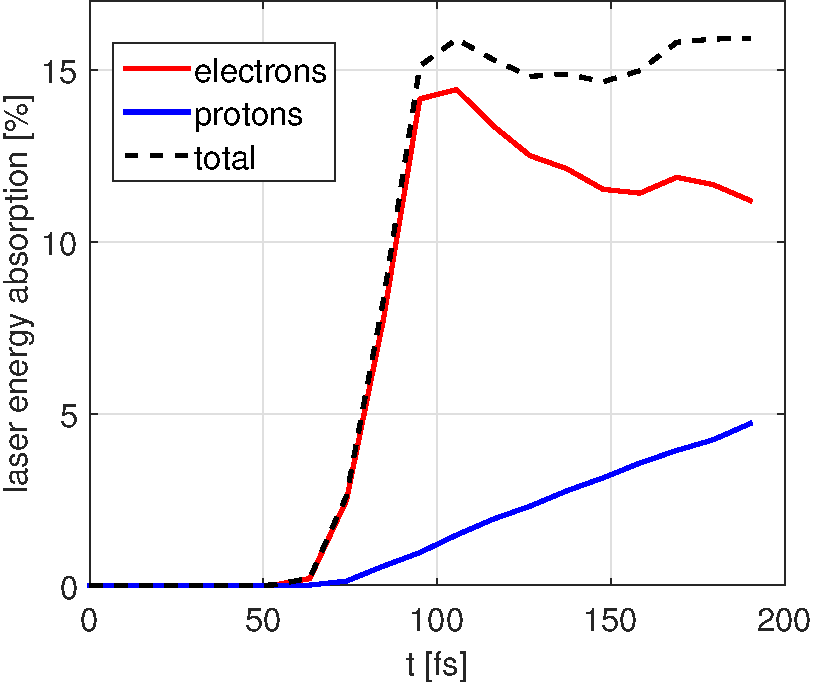
\includegraphics[width=0.45\linewidth]{./img/results/i1e20/05/absorp.pdf}}}
	\sidesubfloat[]{{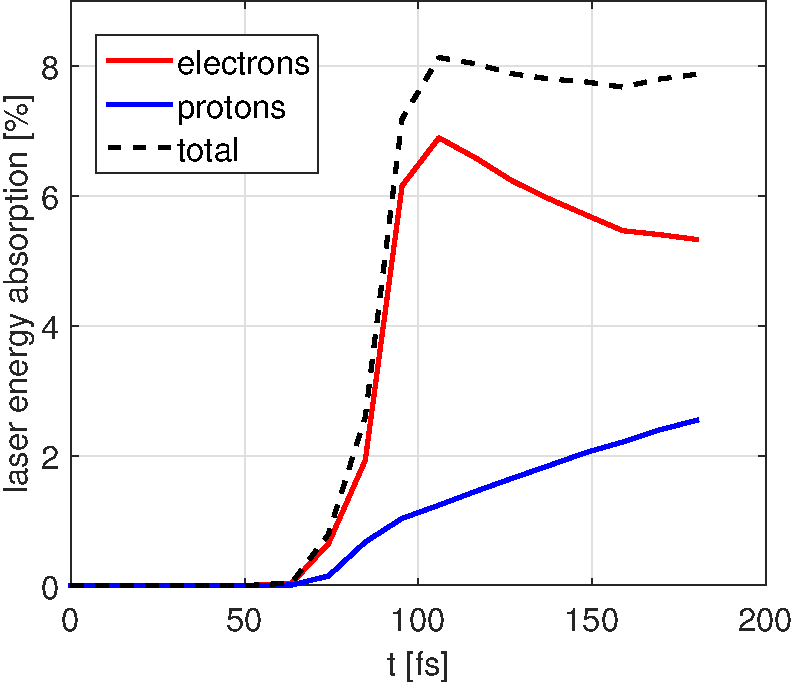
\includegraphics[width=0.45\linewidth]{./img/results/i1e20/2/absorp.pdf}}}\\
	\sidesubfloat[]{{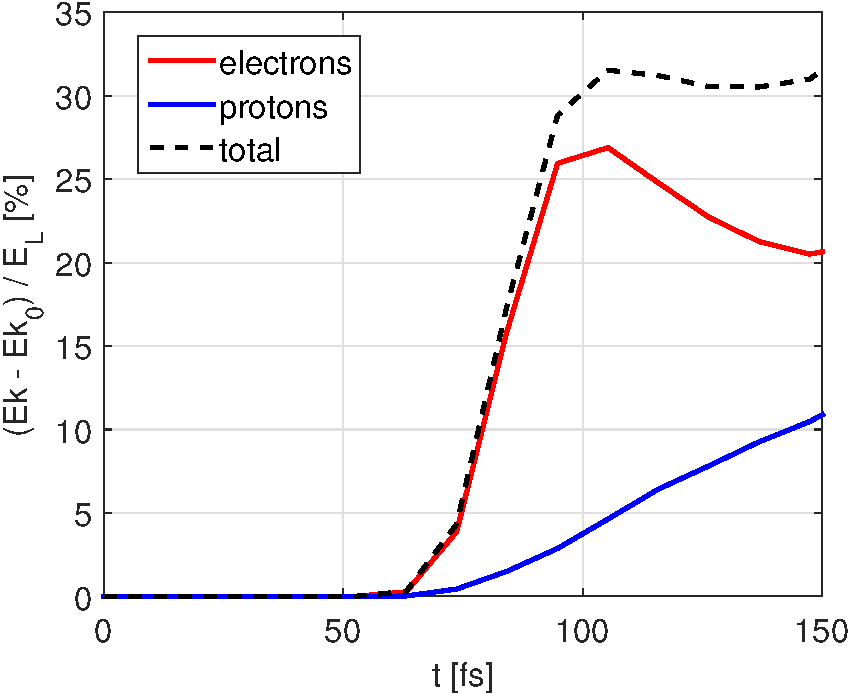
\includegraphics[width=0.45\linewidth]{./img/results/i1e21/05/absorp.pdf}}}
	\sidesubfloat[]{{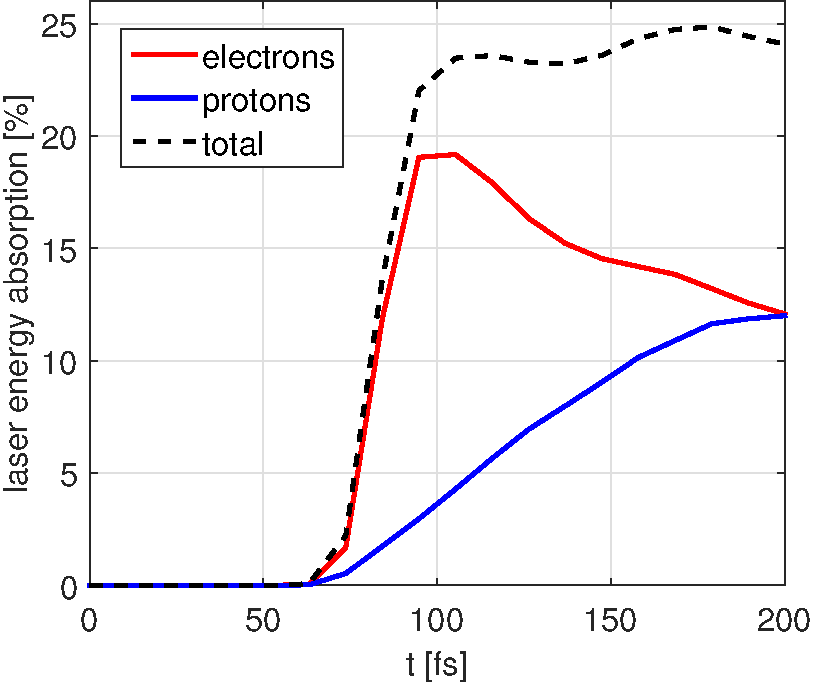
\includegraphics[width=0.45\linewidth]{./img/results/i1e21/2/absorp.pdf}}}
	\caption{\textbf{(a)} w0 = 05 micron, I = 1e20 W/cm2 \textbf{(b)} w0 = 2 micron, I = 1e20 W/cm2 \textbf{(c)} w0 = 05 micron, I = 1e21 W/cm2 \textbf{(d)} w0 = 2 micron, I = 1e21 W/cm2}
	\label{}
\end{figure}

\floatsetup[figure]{style=plain, subcapbesideposition=top}
\begin{figure}[h!]
	\centering
	\sidesubfloat[]{{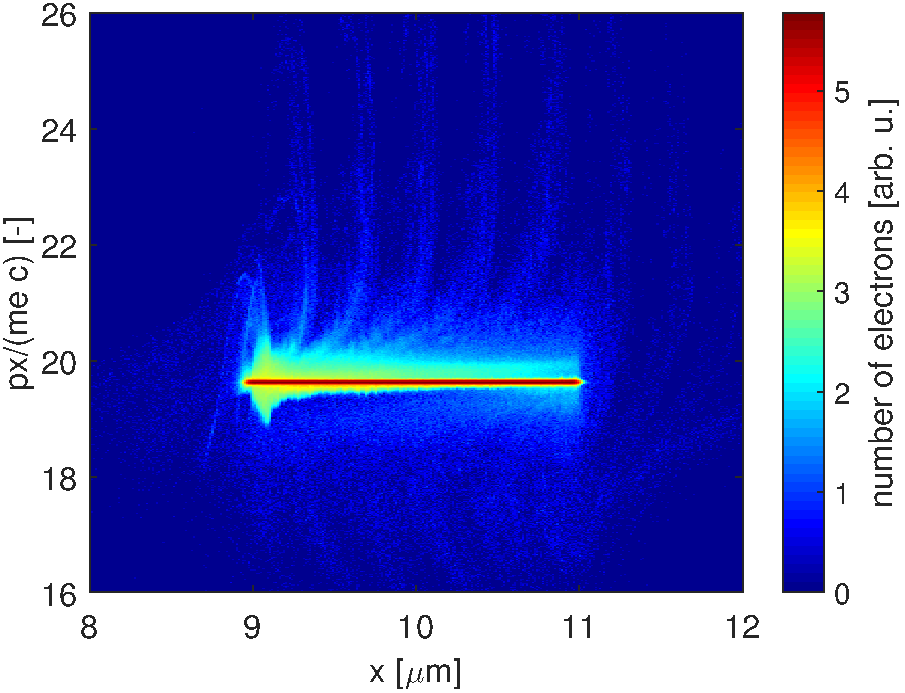
\includegraphics[width=0.45\linewidth]{./img/results/i1e20/05/x_px.pdf}}}
	\sidesubfloat[]{{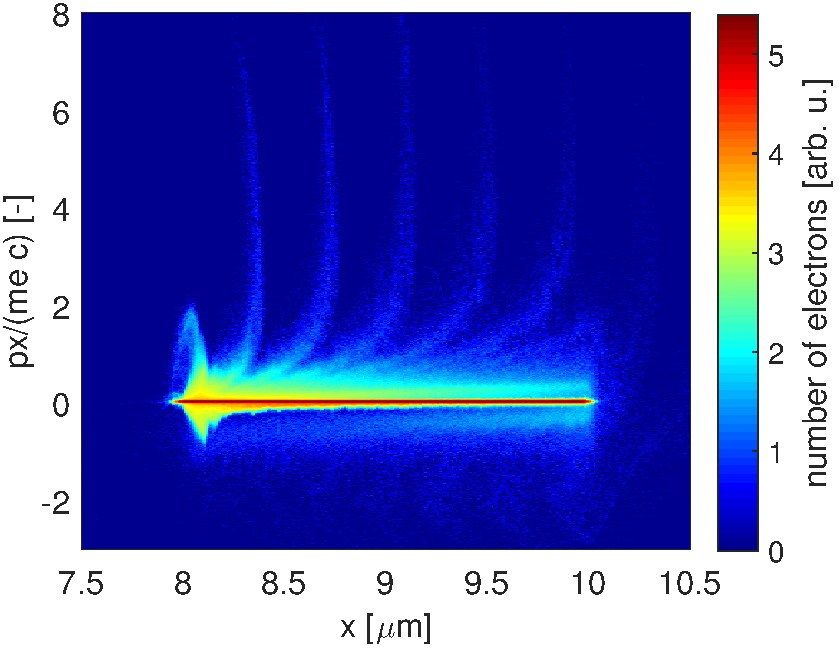
\includegraphics[width=0.45\linewidth]{./img/results/i1e20/2/x_px.pdf}}}\\
	\sidesubfloat[]{{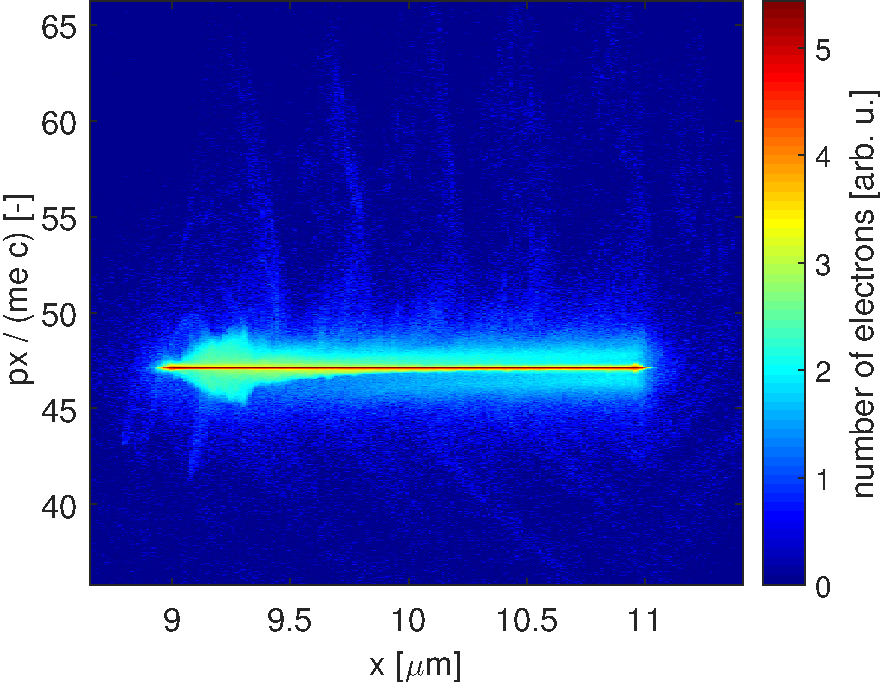
\includegraphics[width=0.45\linewidth]{./img/results/i1e21/05/x_px.pdf}}}
	\sidesubfloat[]{{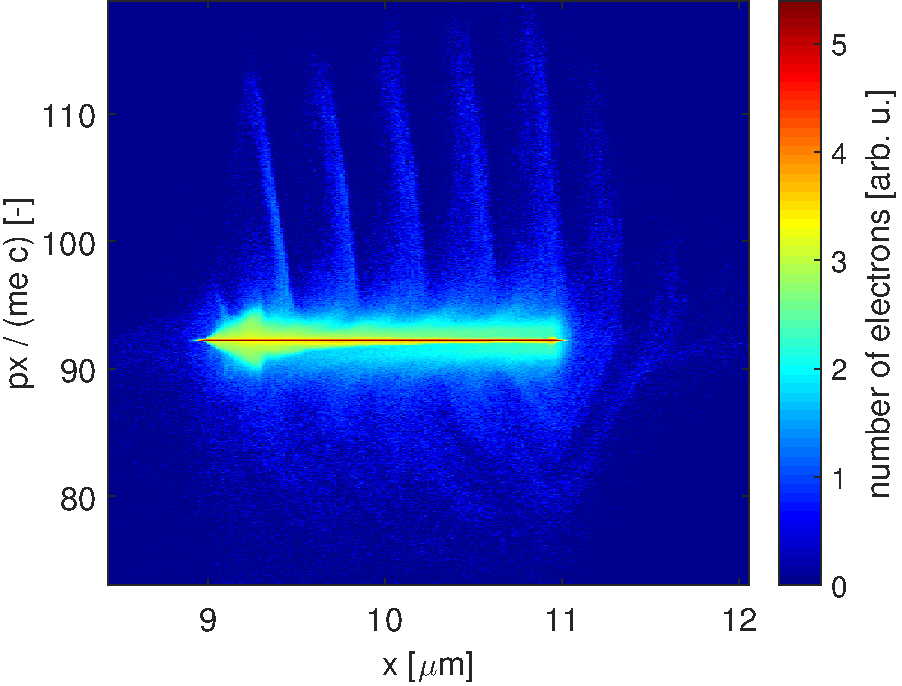
\includegraphics[width=0.45\linewidth]{./img/results/i1e21/2/x_px.pdf}}}
	\caption{\textbf{(a)} w0 = 05 micron, I = 1e20 W/cm2, t = 100 fs \textbf{(b)} w0 = 2 micron, I = 1e20 W/cm2, t = 100 fs \textbf{(c)} w0 = 05 micron, I = 1e21 W/cm2, t = 100 fs \textbf{(d)} w0 = 2 micron, I = 1e21 W/cm2, t = 100 fs}
	\label{}
\end{figure}

\floatsetup[figure]{style=plain, subcapbesideposition=top}
\begin{figure}[h!]
	\centering
	\sidesubfloat[]{{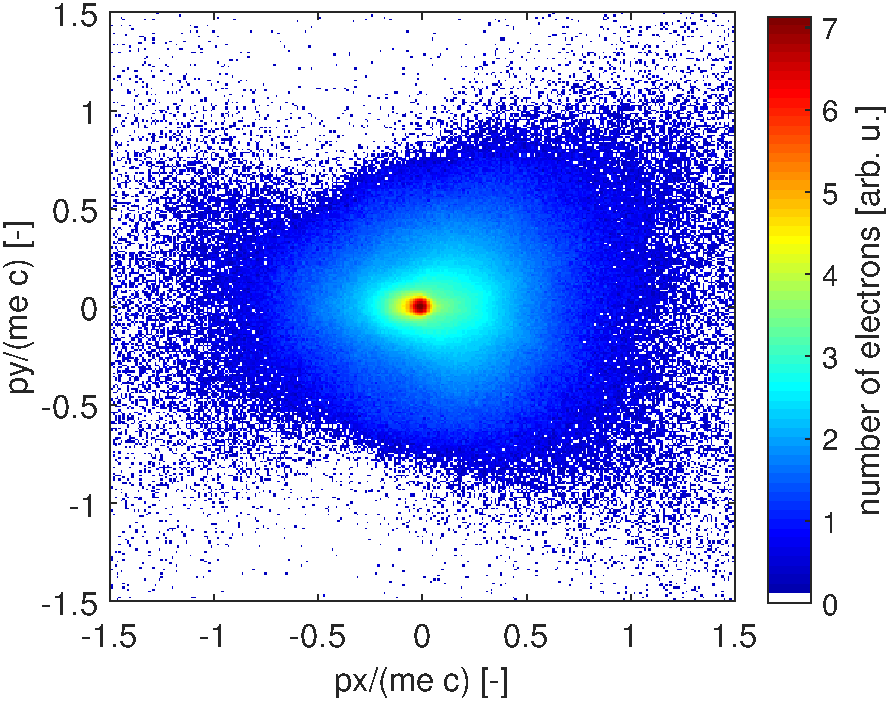
\includegraphics[width=0.45\linewidth]{./img/results/i1e20/05/px_py.pdf}}}
	\sidesubfloat[]{{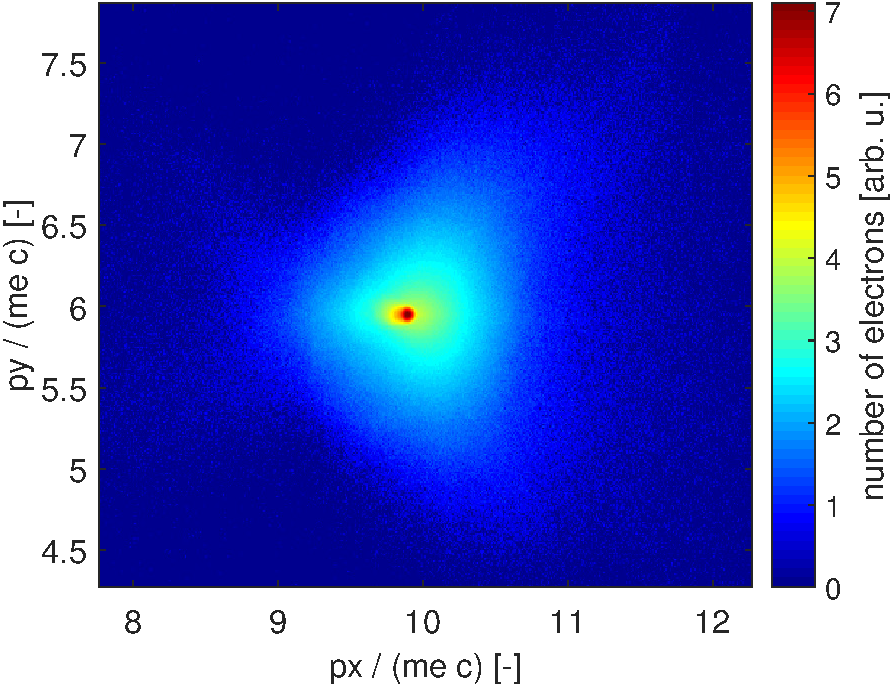
\includegraphics[width=0.45\linewidth]{./img/results/i1e20/2/px_py.pdf}}}\\
	\sidesubfloat[]{{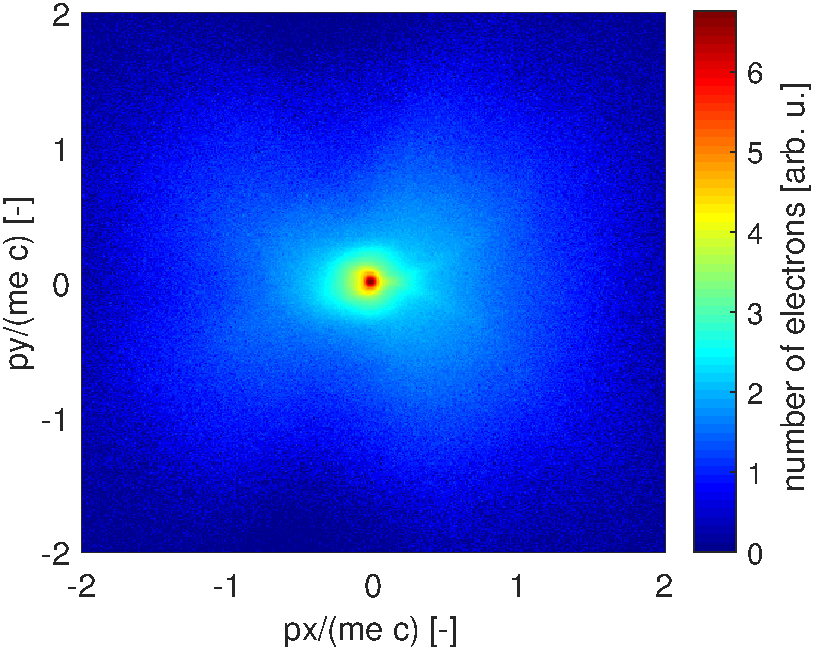
\includegraphics[width=0.45\linewidth]{./img/results/i1e21/05/px_py.pdf}}}
	\sidesubfloat[]{{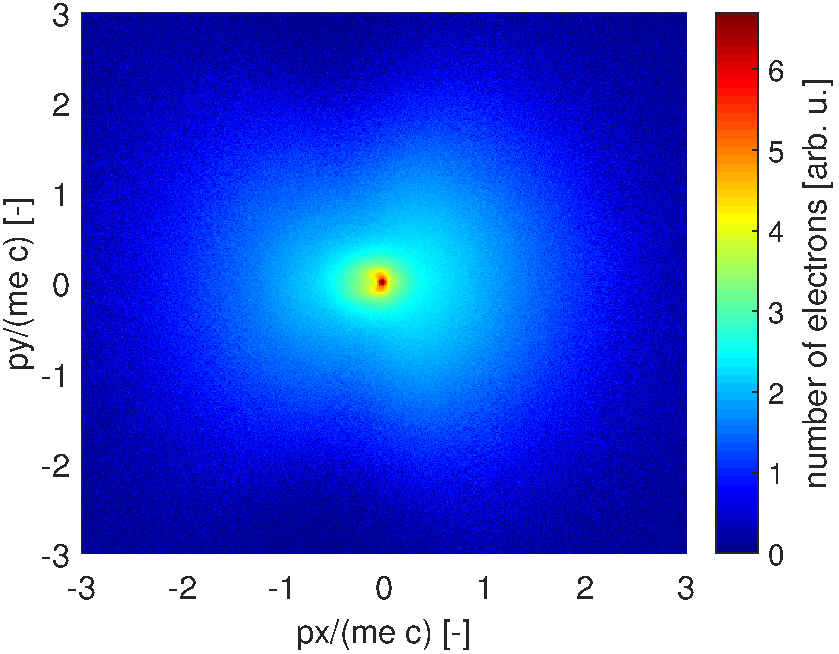
\includegraphics[width=0.45\linewidth]{./img/results/i1e21/2/px_py.pdf}}}
	\caption{\textbf{(a)} w0 = 05 micron, I = 1e20 W/cm2, t = 100 fs \textbf{(b)} w0 = 2 micron, I = 1e20 W/cm2, t = 100 fs \textbf{(c)} w0 = 05 micron, I = 1e21 W/cm2, t = 100 fs \textbf{(d)} w0 = 2 micron, I = 1e21 W/cm2, t = 100 fs}
	\label{}
\end{figure}

\floatsetup[figure]{style=plain, subcapbesideposition=top}
\begin{figure}[h!]
	\centering
	\sidesubfloat[]{{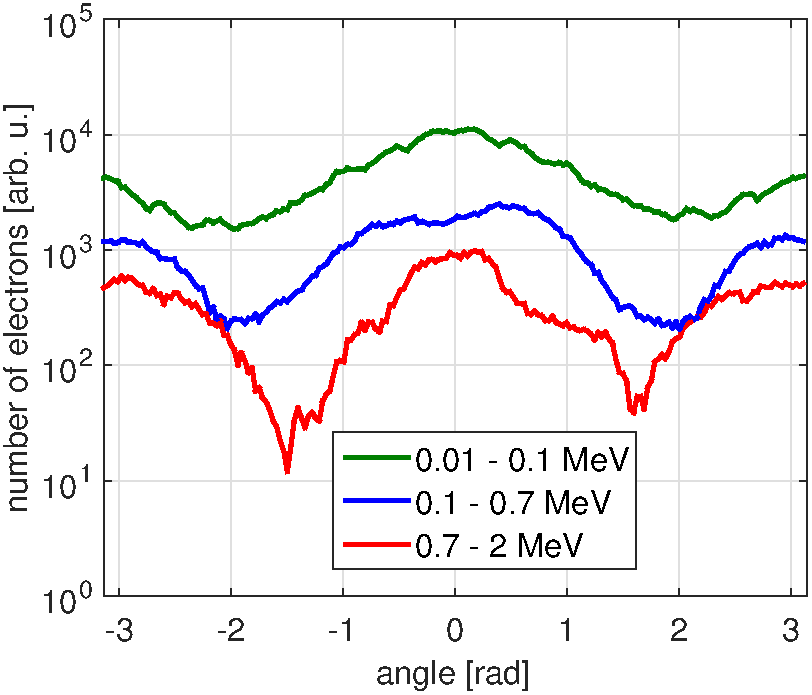
\includegraphics[width=0.445\linewidth]{./img/results/i1e20/05/angles.pdf}}}
	\hspace{1mm}
	\sidesubfloat[]{{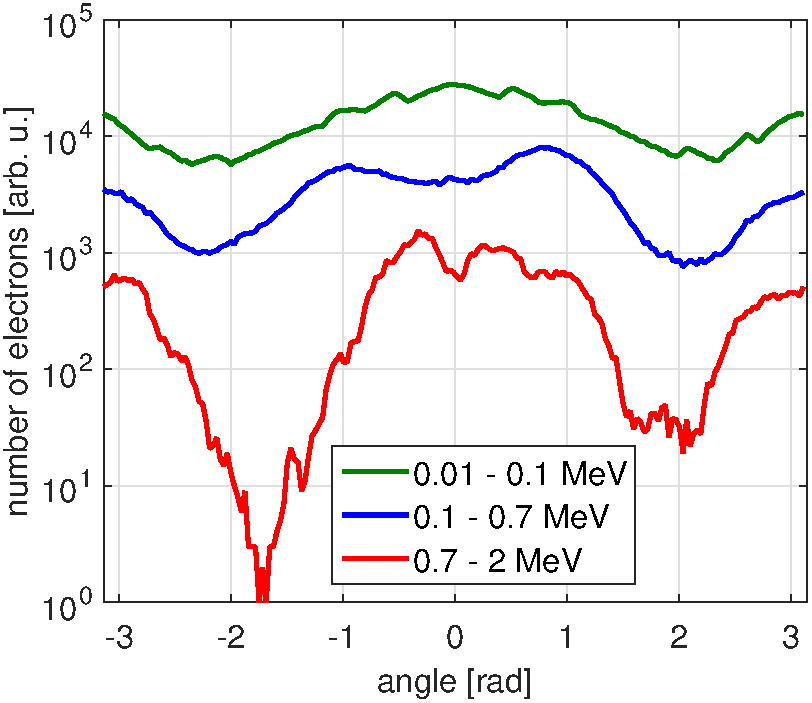
\includegraphics[width=0.445\linewidth]{./img/results/i1e20/2/angles.pdf}}}\\
	\sidesubfloat[]{{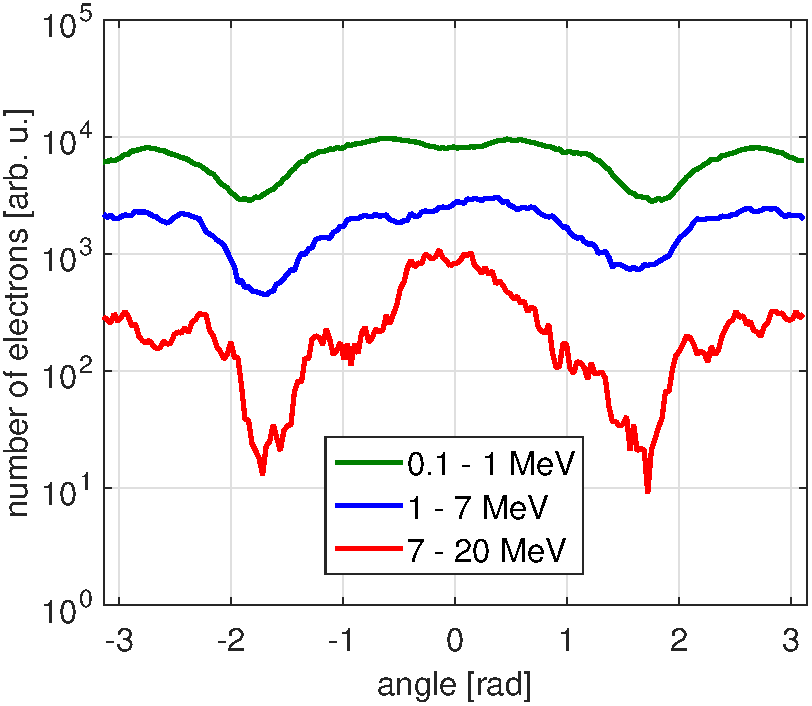
\includegraphics[width=0.445\linewidth]{./img/results/i1e21/05/angles.pdf}}}
	\hspace{1mm}
	\sidesubfloat[]{{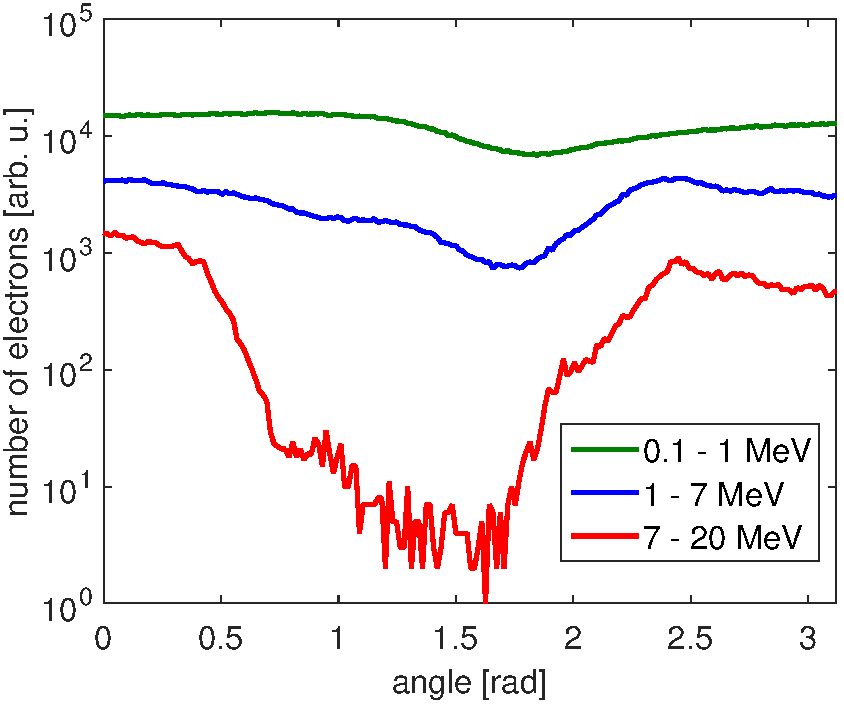
\includegraphics[width=0.445\linewidth]{./img/results/i1e21/2/angles.pdf}}}
	\caption{}
	\label{}
\end{figure}

\floatsetup[figure]{style=plain, subcapbesideposition=top}
\begin{figure}[h!]
	\centering
	\sidesubfloat[]{{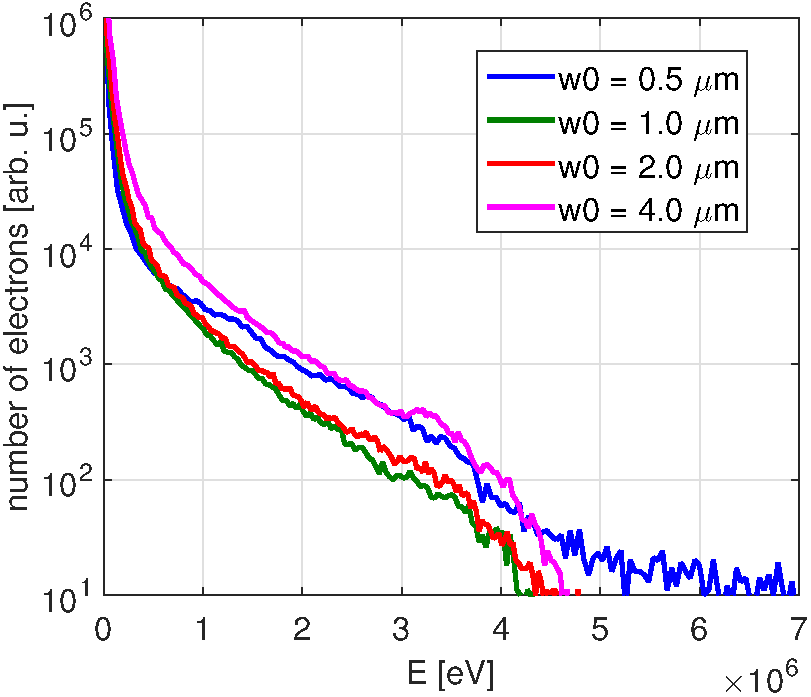
\includegraphics[width=0.445\linewidth]{./img/results/i1e20/dist_e.pdf}}}
	\hspace{1mm}
	\sidesubfloat[]{{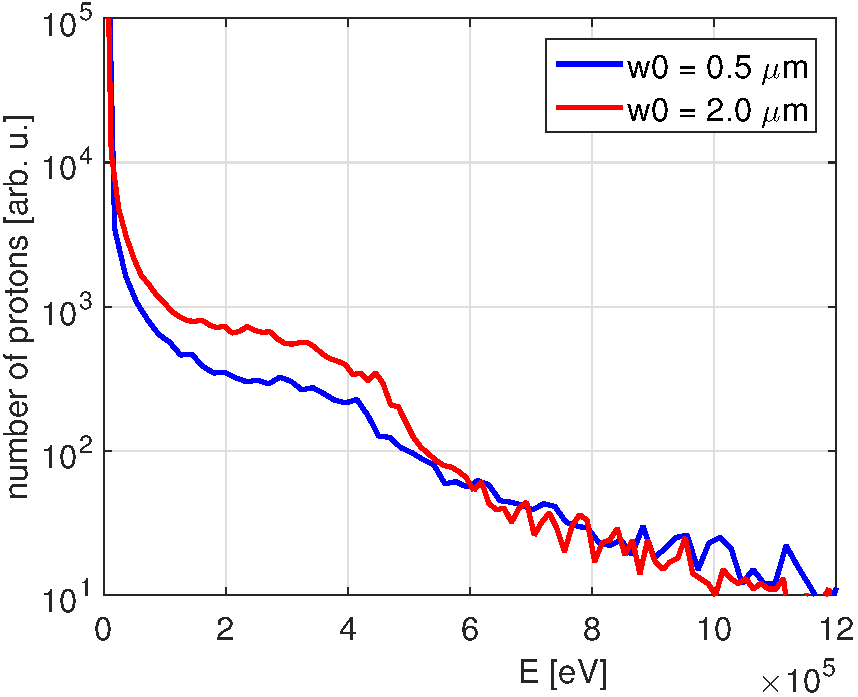
\includegraphics[width=0.445\linewidth]{./img/results/i1e20/dist_p.pdf}}}\\[2mm]
	\sidesubfloat[]{{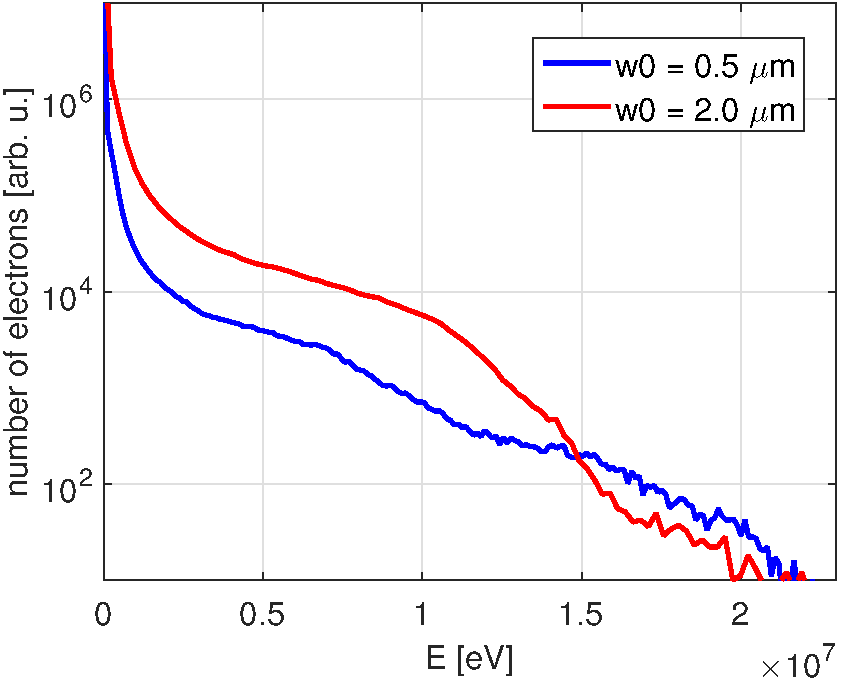
\includegraphics[width=0.445\linewidth]{./img/results/i1e21/dist_e.pdf}}}
	\hspace{1mm}
	\sidesubfloat[]{{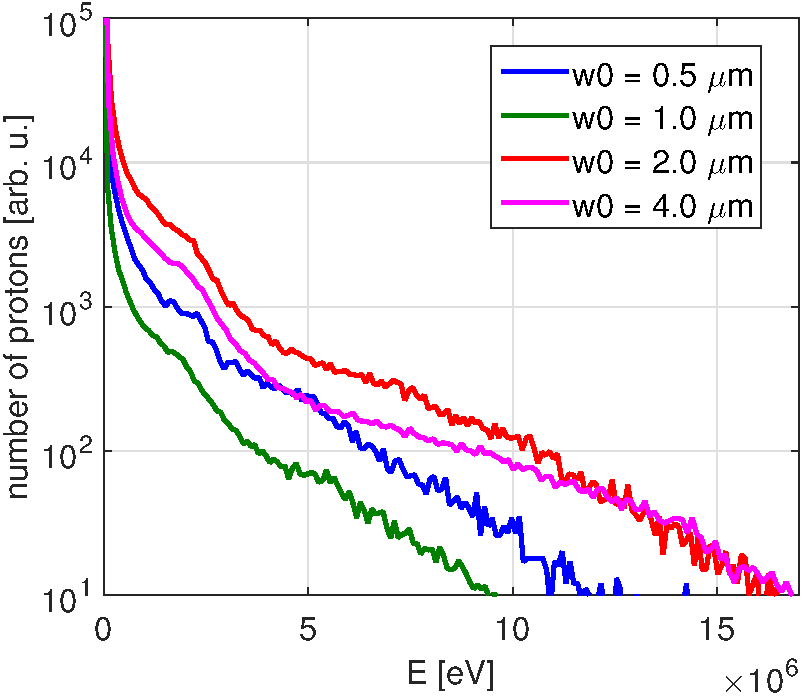
\includegraphics[width=0.445\linewidth]{./img/results/i1e21/dist_p.pdf}}}
	\caption{}
	\label{}
\end{figure}

\floatsetup[figure]{style=plain, subcapbesideposition=top}
\begin{figure}[h!]
	\centering
	\sidesubfloat[]{{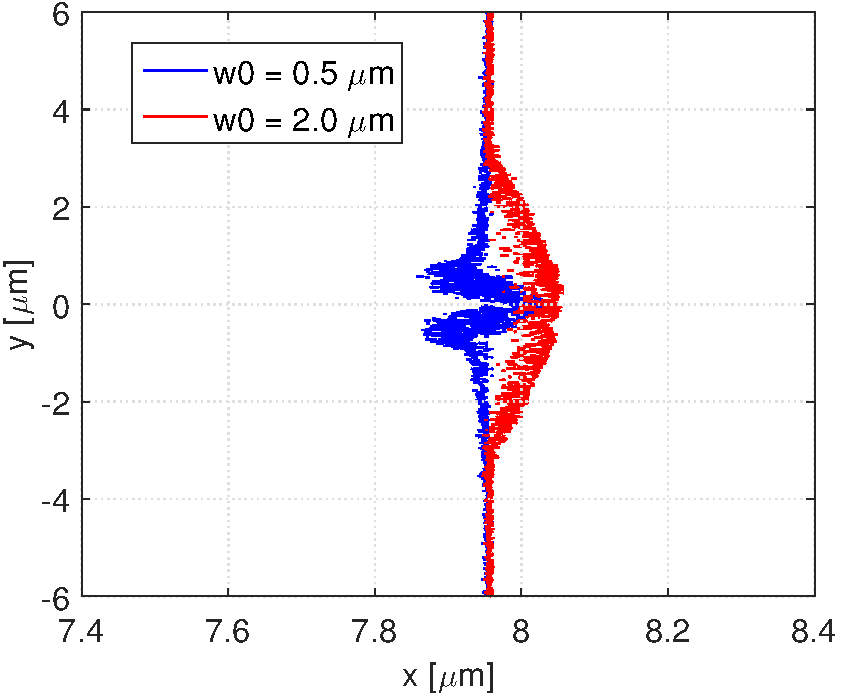
\includegraphics[width=0.445\linewidth]{./img/results/i1e20/dens.pdf}}}
	\hspace{1mm}
	\sidesubfloat[]{{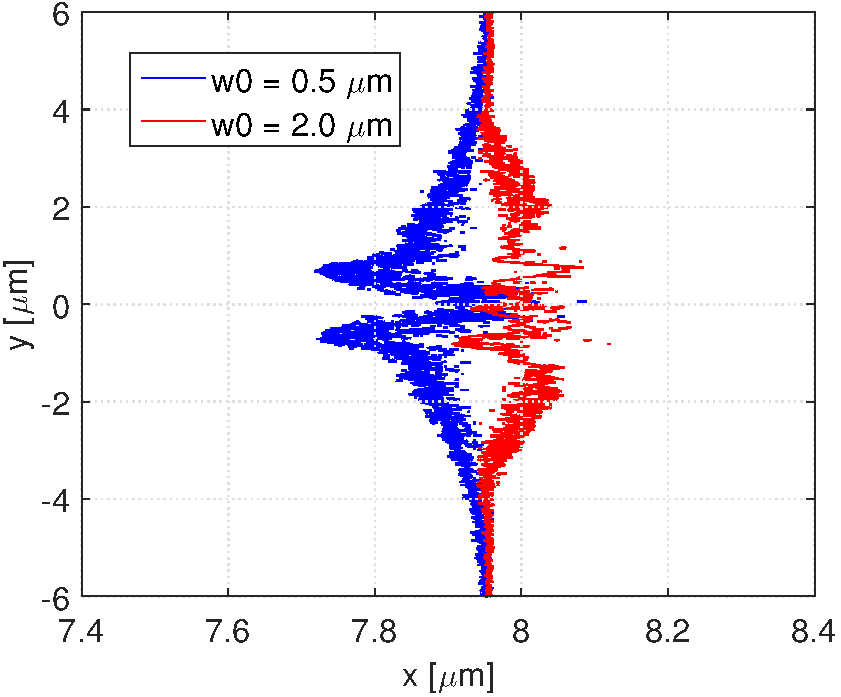
\includegraphics[width=0.445\linewidth]{./img/results/i1e21/dens.pdf}}}
	\caption{\textbf{(a)} nc protons, t = 100 fs, I = 1e20 W/cm2 \textbf{(b)} nc protons, t = 100 fs, I = 1e21 W/cm2}
	\label{}
\end{figure}

\floatsetup[figure]{style=plain, subcapbesideposition=top}
\begin{figure}[h!]
	\centering
	\sidesubfloat[]{{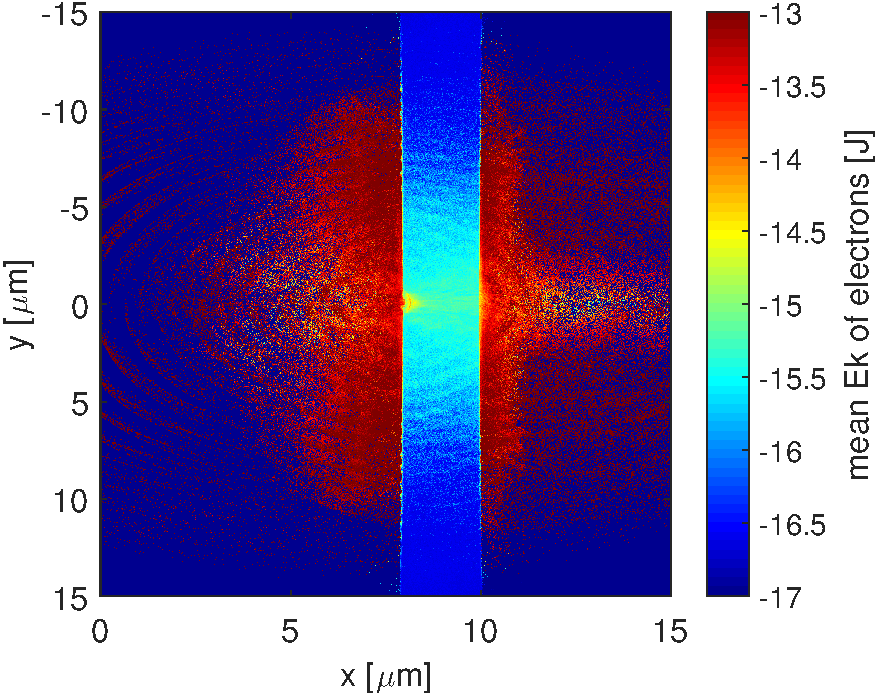
\includegraphics[width=0.45\linewidth]{./img/results/i1e20/05/ekbar.pdf}}}
	\sidesubfloat[]{{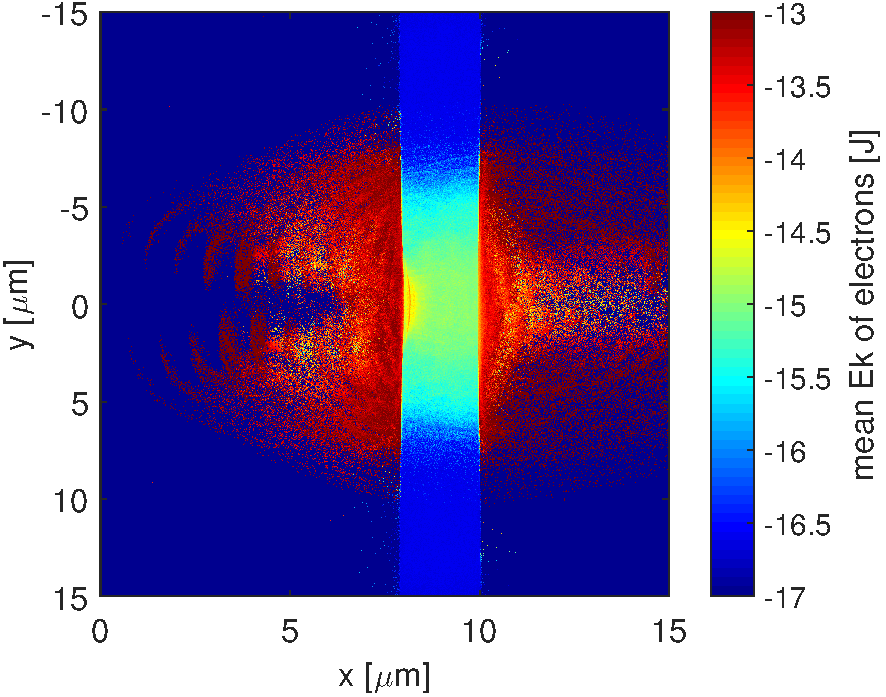
\includegraphics[width=0.45\linewidth]{./img/results/i1e20/2/ekbar.pdf}}}\\[2mm]
	\sidesubfloat[]{{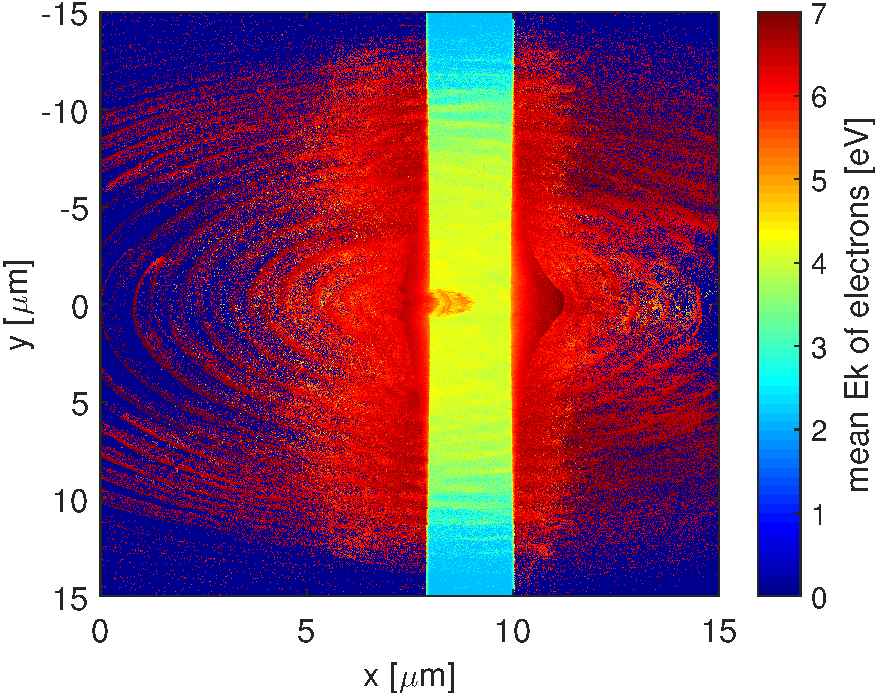
\includegraphics[width=0.45\linewidth]{./img/results/i1e21/05/ekbar.pdf}}}
	\sidesubfloat[]{{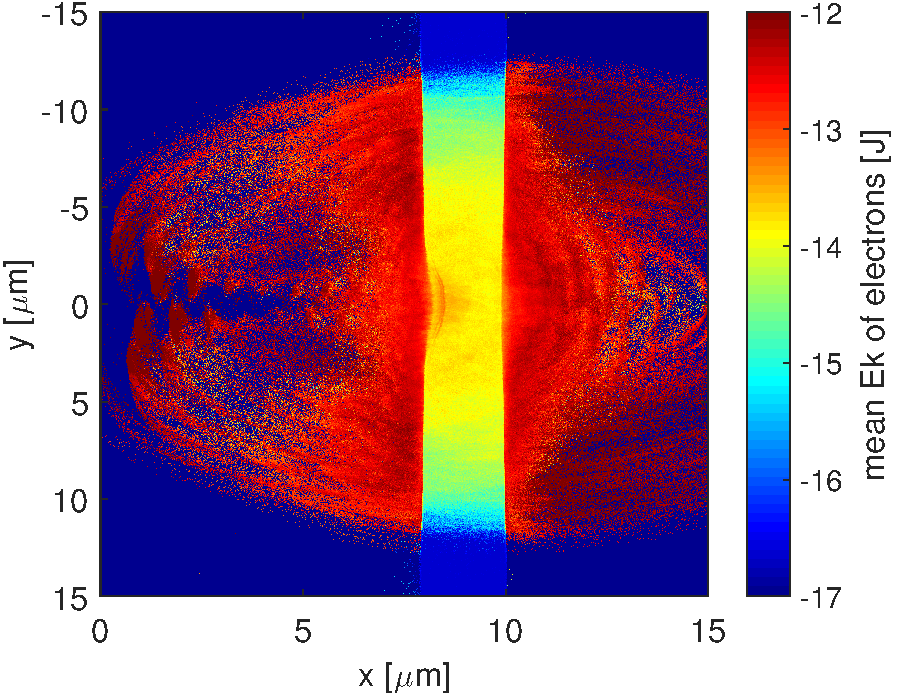
\includegraphics[width=0.45\linewidth]{./img/results/i1e21/2/ekbar.pdf}}}
	\caption{}
	\label{}
\end{figure}

\floatsetup[figure]{style=plain, subcapbesideposition=top}
\begin{figure}[h!]
	\centering
	\sidesubfloat[]{{\includegraphics[width=0.45\linewidth]{./img/results/i1e20/05/abs_ex.pdf}}}
	\sidesubfloat[]{{\includegraphics[width=0.45\linewidth]{./img/results/i1e20/2/abs_ex.pdf}}}\\[2mm]
	\sidesubfloat[]{{\includegraphics[width=0.45\linewidth]{./img/results/i1e21/05/abs_ex.pdf}}}
	\sidesubfloat[]{{\includegraphics[width=0.45\linewidth]{./img/results/i1e21/2/abs_ex.pdf}}}
	\caption{}
	\label{}
\end{figure}

\floatsetup[figure]{style=plain, subcapbesideposition=top}
\begin{figure}[h!]
	\centering
	\sidesubfloat[]{{\includegraphics[width=0.45\linewidth]{./img/results/i1e20/05/fpx.pdf}}}
	\sidesubfloat[]{{\includegraphics[width=0.45\linewidth]{./img/results/i1e20/05/fpy.pdf}}}\\
	\sidesubfloat[]{{\includegraphics[width=0.45\linewidth]{./img/results/i1e20/2/fpx.pdf}}}
	\sidesubfloat[]{{\includegraphics[width=0.45\linewidth]{./img/results/i1e20/2/fpy.pdf}}}
	\caption{\textbf{(a)} 5.1312e-06 \textbf{(b)} 1.5913e-06 \textbf{(c)} 5.9528e-06 \textbf{(d)} 4.6193e-07}
	\label{}
\end{figure}